\subsection{28.07.08 - Surface Work}

\begin{marginfigure}
\checkoddpage \ifoddpage \forcerectofloat \else \forceversofloat \fi
\centering
 \frame{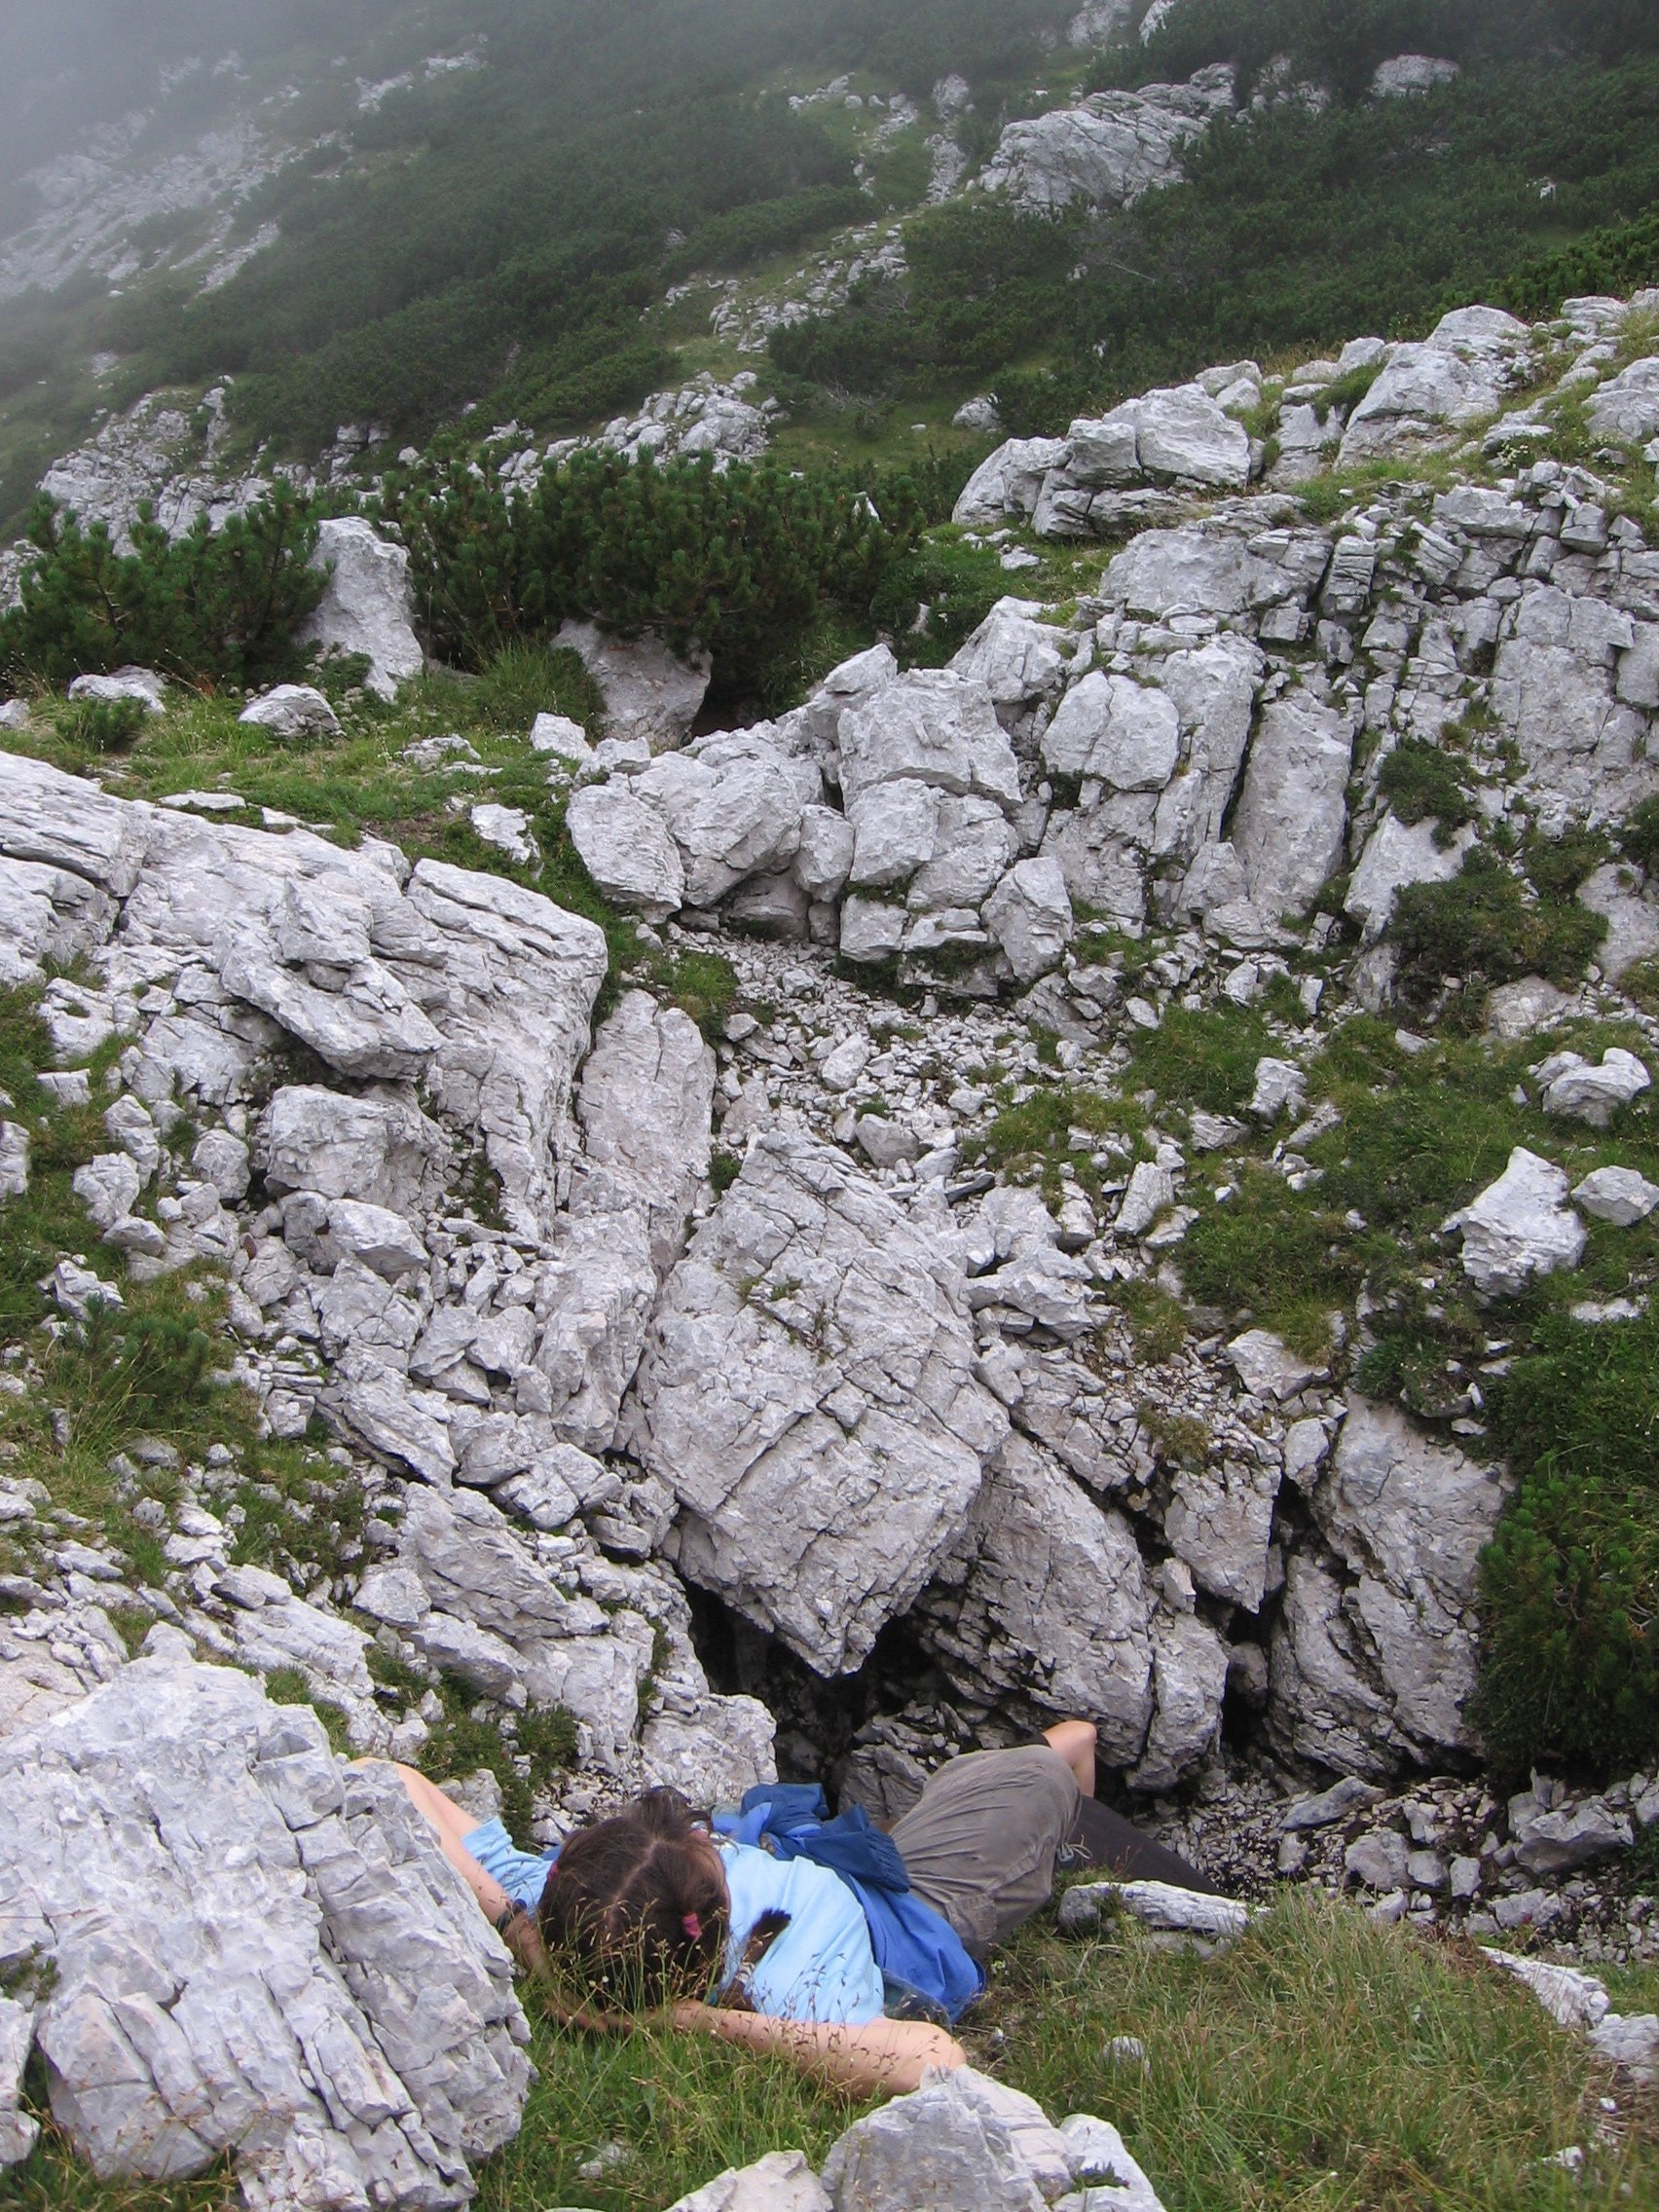
\includegraphics[width=\linewidth]{2008/surface/Jarvist Frost - canon a520 -janet lounging near new cave on plateau below mig--orig.jpg}} 
 \caption{Janet demonstrates the pleasures of surface bashing. \pic{Jarvist Frost}}
 \label{janet relax}
\end{marginfigure}




\begin{enumerate}
\def\labelenumi{\arabic{enumi}.}
% \tightlist
\item
  Went back to Valley 8 (next one to \passage{B9}), you can see loads of cave
  entrances. Check out. But only one goes. You climb down under the
  boulder choke, turn right down to a small chamber. From here there are
  at least 2 ways on. They both require the removal of boulders. All to
  be done very gently and carefully since so many blocks hang on top,
  but otherwise looking good to go.
\item
  Behind \passage{M19} have noticed a small cave entrance. A slope down to a
  chamber visible. Did not go down, since at that time I was alone. Put
  a cairn to mark an entrance.
\item
  East of \passage{M19} possibly next to \passage{M15} - There is a big
  entrance. We climbed down and digged (a bit) 3 possible routes on.
  Quite draughty. On to the bottom way on(?) we noticed that someone
  might have used a hammer. You can feel a lot of cold draught. Digging,
  smashing, needed but it does look very good to go!
  \sidenote{JCC GPS Waypoint 1851 m N46.25311 E013.7610}
\item
  Loads of big (deep) entrances just behind the Bivi. Almost of them
  have snow at the bottom. Rope needed to explore!
\item
  Re-discover the \passage{Royston Vasey} (we believe?) re-located.
  \sidenote{See Hollow Mountain I, p. 147}
\item
  Re-discover, located a cave entrance with a red spot in front. It
  starts with a narrow pitch down. Next to red spot it is an old bolt as
  well. It is just further on on the right up from \passage{Royston Vasey},
  looking towards \passage{Kuk}. Worth going back down again. (We believe this
  is Dave Wilson's 1996 Dig\sidenote{See Hollow Mountain page XXXXXXXXXXXXXXXXXXXXXXXX})
\end{enumerate}

\name{Jana Čarga}

\fullwidthbox{30-07-08 Jana, Andy, Janet → Surface Work}{

    Jana, Andy and Janet collected the GPS coordinates of all large holes in the area of the Bivi.
    
    They checked the 'M'holes (\passage{M1}, \passage{M16}, \passage{M18}, \passage{M4}, \passage{M15}, \passage{M17}, \passage{M19}), and added new entrances, (\passage{A1} to \passage{A4}), all of which are worth a quick 'go down' and 'look'.
    
    Bolting kits needed!
    
\name{Jana}
}
